% This is "sig-alternate.tex" V2.1 April 2013
% This file should be compiled with V2.5 of "sig-alternate.cls" May 2012
%
% This example file demonstrates the use of the 'sig-alternate.cls'
% V2.5 LaTeX2e document class file. It is for those submitting
% articles to ACM Conference Proceedings WHO DO NOT WISH TO
% STRICTLY ADHERE TO THE SIGS (PUBS-BOARD-ENDORSED) STYLE.
% The 'sig-alternate.cls' file will produce a similar-looking,
% albeit, 'tighter' paper resulting in, invariably, fewer pages.
%
% ----------------------------------------------------------------------------------------------------------------
% This .tex file (and associated .cls V2.5) produces:
%       1) The Permission Statement
%       2) The Conference (location) Info information
%       3) The Copyright Line with ACM data
%       4) NO page numbers
%
% as against the acm_proc_article-sp.cls file which
% DOES NOT produce 1) thru' 3) above.
%
% Using 'sig-alternate.cls' you have control, however, from within
% the source .tex file, over both the CopyrightYear
% (defaulted to 200X) and the ACM Copyright Data
% (defaulted to X-XXXXX-XX-X/XX/XX).
% e.g.
% \CopyrightYear{2007} will cause 2007 to appear in the copyright line.
% \crdata{0-12345-67-8/90/12} will cause 0-12345-67-8/90/12 to appear in the copyright line.
%
% ---------------------------------------------------------------------------------------------------------------
% This .tex source is an example which *does* use
% the .bib file (from which the .bbl file % is produced).
% REMEMBER HOWEVER: After having produced the .bbl file,
% and prior to final submission, you *NEED* to 'insert'
% your .bbl file into your source .tex file so as to provide
% ONE 'self-contained' source file.
%
% ================= IF YOU HAVE QUESTIONS =======================
% Questions regarding the SIGS styles, SIGS policies and
% procedures, Conferences etc. should be sent to
% Adrienne Griscti (griscti@acm.org)
%
% Technical questions _only_ to
% Gerald Murray (murray@hq.acm.org)
% ===============================================================
%
% For tracking purposes - this is V2.0 - May 2012

\documentclass{sig-alternate-05-2015}


\begin{document}

% Copyright
\setcopyright{acmcopyright}
%\setcopyright{acmlicensed}
%\setcopyright{rightsretained}
%\setcopyright{usgov}
%\setcopyright{usgovmixed}
%\setcopyright{cagov}
%\setcopyright{cagovmixed}


% DOI
\doi{10.475/123_4}

% ISBN
\isbn{123-4567-24-567/08/06}

%Conference
\conferenceinfo{OpenSym '16}{August 19--21, 2016, Berlin, Germany}

\acmPrice{\$15.00}

%
% --- Author Metadata here ---
\conferenceinfo{OpenSym}{'16 Berlin, Germany}
%\CopyrightYear{2007} % Allows default copyright year (20XX) to be over-ridden - IF NEED BE.
%\crdata{0-12345-67-8/90/01}  % Allows default copyright data (0-89791-88-6/97/05) to be over-ridden - IF NEED BE.
% --- End of Author Metadata ---

\title{Determining the Geographical distribution of a Community by means
of a Time-zone Analysis}
%\subtitle{[Extended Abstract]
%\titlenote{A full version of this paper is available as
%\textit{Author's Guide to Preparing ACM SIG Proceedings Using
%\LaTeX$2_\epsilon$\ and BibTeX} at
%\texttt{www.acm.org/eaddress.htm}}}
%
% You need the command \numberofauthors to handle the 'placement
% and alignment' of the authors beneath the title.
%
% For aesthetic reasons, we recommend 'three authors at a time'
% i.e. three 'name/affiliation blocks' be placed beneath the title.
%
% NOTE: You are NOT restricted in how many 'rows' of
% "name/affiliations" may appear. We just ask that you restrict
% the number of 'columns' to three.
%
% Because of the available 'opening page real-estate'
% we ask you to refrain from putting more than six authors
% (two rows with three columns) beneath the article title.
% More than six makes the first-page appear very cluttered indeed.
%
% Use the \alignauthor commands to handle the names
% and affiliations for an 'aesthetic maximum' of six authors.
% Add names, affiliations, addresses for
% the seventh etc. author(s) as the argument for the
% \additionalauthors command.
% These 'additional authors' will be output/set for you
% without further effort on your part as the last section in
% the body of your article BEFORE References or any Appendices.

\numberofauthors{3} %  in this sample file, there are a *total*
% of EIGHT authors. SIX appear on the 'first-page' (for formatting
% reasons) and the remaining two appear in the \additionalauthors section.
%
\author{
% You can go ahead and credit any number of authors here,
% e.g. one 'row of three' or two rows (consisting of one row of three
% and a second row of one, two or three).
%
% The command \alignauthor (no curly braces needed) should
% precede each author name, affiliation/snail-mail address and
% e-mail address. Additionally, tag each line of
% affiliation/address with \affaddr, and tag the
% e-mail address with \email.
%
% 1st. author
\alignauthor
Jesus M. Gonzalez-Barahona\\
       \affaddr{Universidad Rey Juan Carlos}\\
       \affaddr{Madrid, Spain}\\
       \email{jgb@gsyc.urjc.es}
% 2nd. author
\alignauthor
Gregorio Robles\\
       \affaddr{Universidad Rey Juan Carlos}\\
       \affaddr{Madrid, Spain}\\
       \email{grex@gsyc.urjc.es}
% 3rd. author
\alignauthor
Daniel Izquierdo-Cortazar\\
       \affaddr{Bitergia}\\
       \affaddr{Madrid, Spain}\\
       \email{dizquierdo@bitergia.com}
}
% There's nothing stopping you putting the seventh, eighth, etc.
% author on the opening page (as the 'third row') but we ask,
% for aesthetic reasons that you place these 'additional authors'
% in the \additional authors block, viz.
%\additionalauthors{Additional authors: John Smith (The Th{\o}rv{\"a}ld Group,
%%email: {\texttt{jsmith@affiliation.org}}) and Julius P.~Kumquat
%(The Kumquat Consortium, email: {\texttt{jpkumquat@consortium.net}}).}
%\date{30 July 1999}
% Just remember to make sure that the TOTAL number of authors
% is the number that will appear on the first page PLUS the
% number that will appear in the \additionalauthors section.

\maketitle
\begin{abstract}
Free/libre/open source software projects are usually developed by a geographically distributed community of developers and contributors. In contrast to traditional corporate environments, it is hard to obtain information about how the community is geographically distributed, mainly because participation is open to volunteers and in many cases it is just occasional. During the last years, specially with the increasing implication of institutions, non-profit organizations and companies, there is a growing interest in having information about the geographic location of developers. This is because projects want to be as global as possible, in order to attract new contributors, users and, of course, clients. In this
paper we show a methodology to obtain the geographical distribution of a development community by analyzing the source code management system and the mailing lists they use.
\end{abstract}


%
% The code below should be generated by the tool at
% http://dl.acm.org/ccs.cfm
% Please copy and paste the code instead of the example below. 
%

\begin{CCSXML}
<ccs2012>
<concept>
<concept_id>10003120.10003130</concept_id>
<concept_desc>Human-centered computing~Collaborative and social computing</concept_desc>
<concept_significance>500</concept_significance>
</concept>
</ccs2012>
\end{CCSXML}

\ccsdesc[500]{Human-centered computing~Collaborative and social computing}

%
% End generated code
%

%
%  Use this command to print the description
%
\printccsdesc

% We no longer use \terms command
%\terms{Theory}

\keywords{FLOSS; distributed development; time zones; open source software;}


%-----------------------------------------------------------------------
\section{Introduction}
\label{sec:intro}

Although free/libre/open source software (FLOSS) can be produced in many different ways, it is common practice nowadays that it is developed by a geographically distributed community. In this case, developers and other kinds of contributors share code, suggestions, comments, bug reports and discussions on the Internet, using specific-purpose communication and development tools. These communities have been subject of many research studies, some of them focusing on how they manage to work in a distributed manner~\cite{german2003gnome,yu2016effect}.

As communities have become more organized and institutionalized themselves, may it be through the creation of foundations or other legal entities~\cite{riehle2010economic}, or with the growing interest in FLOSS by industrial companies, the information of where developers, contributors and users are has gained more importance. Some communities have shown interest to include such type of information in their software development dashboards\footnote{For example, dashboards for some communities offered by Bitergia, the company, can be found at \url{http://bitergia.com/dashboards/}.}.

An example of a community with a long lasting interest in learning about the geographic information of its developers is Debian. The Debian project maintains a map with the location of their developers\footnote{\url{https://www.debian.org/devel/developers.loc}}. %(see figure~\ref{fig:debian-map}),
It shows how Debian is an international project, primarily based in Western countries, with a certain balance between the number of North American and European developers. This is an interesting fact, for example, to choose the location of the DebConf, the annual Debian conference. It is also useful for Debian applicants to locate developers geographically close to them, since their admission process~\cite{robles2005evolution} requires face-to-face contact (for instance,
to get the RSA key signed by an already Debian developer). 

%\begin{figure}[!h]
%\centering
%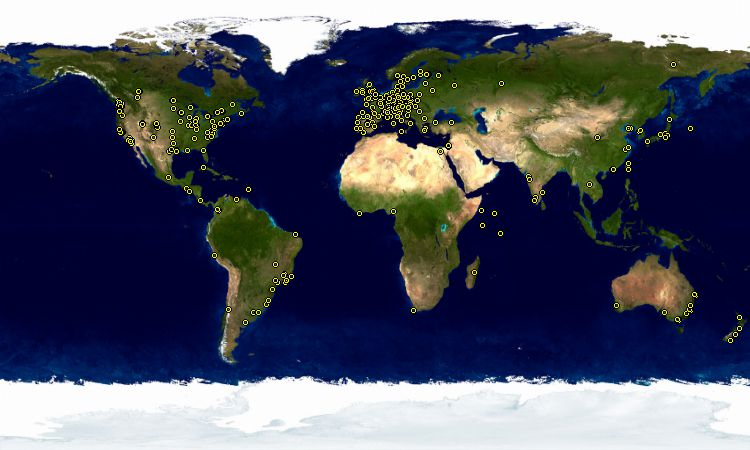
\includegraphics[width=8cm]{figs/developers-map}
%\caption{Map with the geographical location of Debian developers (as of 
%January 2015).}
%\label{fig:debian-map}
%\end{figure}

As another case, Mozilla's mission states that they want that ``people worldwide can be informed contributors and creators of the Web''\footnote{\url{https://www.mozilla.org/en-US/mission/}}, so information about virtual participation is useful to design a global strategy. This type of information can be used as well by companies to assess the interest on their FLOSS products iin certain geographic areas, and as information helpful in opening new markets.

But getting this information is not easy in most cases, since there are little data sources to collect it. The goal of this paper is to show a methodology to obtain the geographic distribution of a FLOSS community by means of analyzing artifacts produced as side-product of the software development effort. Therefore data will be extracted from source code management systems (such as Git) and mailing list archives, and don't require the active collaboration of developers.

The structure of the rest of this paper starts with the presentation of related research.
% Section~\ref{sec:questions}
%contains the specific research questions that this paper targets. 
In Section~\ref{sec:methodology}, we detail the proposed methodology. Then we explain how we apply it to analyze the CloudStack project, as an illustrative case study (Section~\ref{sec:case-study}). Results of this application are presented in Section~\ref{sec:results}. Finally, some conclusions are drawn and future directions are discussed.


%-----------------------------------------------------------------------
%\section{Research questions}
%\label{sec:questions}
%
%\begin{enumerate}
%  \item
%
%  \item 
% 
%  \item 
%\end{enumerate}


%-----------------------------------------------------------------------
\section{Related research}
\label{sec:related}

The coordinated development of a software product by geographically distributed
teams has been a matter of study since the late 1990s~\cite{carmel1999global}.
The specific case of FLOSS communities has been considered in several cases~\cite{german2003gnome,engelhardt2009geographic,von2010geographic}, even with some attention to regions where FLOSS developemnt is rare, such as Africa~\cite{ouattara2013open}.

Some of these efforts tried to estimate the location of the global FLOSS development commuunity, such as the study of the geographical data obtained from the accounts of over one million registered users at SourceForge~\cite{robles2006geographic,gonzalez2008geographic}. In other cases, massive surveys were performed~\cite{ghosh2002free,david2008community}. Some of those asked for the country of origin and the current country of residence, in order to find developer migration patterns, finding how talent is attracted by the United States from all over the world~\cite{ghosh2002free}.

The target for this paper is not to obtain an statistical estimate of the global FLOSS community, but to obtain a picture as accurate as possible of the community of a given project. Therefore, instead of performing massive surveys or analyzing software development platforms with many projects, we target project-specific tools. A similar approach can be found in Bird et al. who have examined how two large FLOSS projects perform their work in a distributed manner~\cite{bird2012examining}. Related to the methods used in this paper, Tang et al. propose a set of 
techniques for identifying the country origin of mailing list participants~\cite{tang2009techniques}, which they use to perform a case study on the impact of global participation on mailing lists communications in FLOSS projects~\cite{tang2009case}.

%-----------------------------------------------------------------------
\section{Methodology}
\label{sec:methodology}

This section details the various steps of the empirical process to extract 
geographical information from publicly available repositories. This analysis is 
focused on the traces left by developers in the Git repositories. And this can
be easily extensible to any other data source with geographical log information.

%The results are based on the analysis of the Git repositories. Git is a
%distributed source code management system tool that allow developers to work
%in their own servers. Those changes to the source code, named as commits, can be
%later \emph{merged} or sent for a \emph{code review} process within the community.

Thanks to the distributed design of Git, each commit contains geographical
information, that is the timezone where the change to the source code took place.
That information is either taken from the local system where the developer works or
configured by that developers.
In addition to the timezone, a commit is typically defined by the \emph{author} of the
commit, the \emph{date} with the \emph{timezone}, a list of \emph{touched} files,
a \emph{log message} and others. 

%Those local commits that are later merged into the main branch, also named as \emph{master}.
%And 

%% Threats to validity: cherry pick, local setup of the timezone in the laptops,
%%                      people working around the world.

In detail, the empirical approach is based on the following four steps:

\begin{enumerate}
\item Identification of data sources: this process needs of understanding the
infrastructure of the community or project to analyze. That information is
typically accessible and specified in open source communities. This method
focuses on the development activity, so source code repositories are the
needed ones.

\item Extraction of information from data sources: the data process extraction
is done thanks to the use of
\emph{CVSAnalY}\footnote{\url{https://github.com/MetricsGrimoire/CVSAnalY}}
 a FLOSS data extraction tool that allow us to store in a MySQL
database information coming from Git activity.
%link to the tools for usual bla bla from IJOSSP.

\item Analysis of the dataset: we need then to filter part of the data.
Given the amount of information provided by CVSAnalY, and that not all of
such information is useful for this analysis, several filters can be applied
to the analysis.

In this case, \emph{merge} commits were ignored. The rationale
for this is that merges are in most of the cases automatically done and do not
have more information that the action and the point in time where a merge took place; no source code is modified.

\item Timezone analysis: for this, we took advantage of
\emph{GrimoireLib}\footnote{\url{https://github.com/VizGrimoire/GrimoireLib/}} a library
specialized on the analysis of information structured in SQL databases coming from
\emph{Metrics Grimoire}\footnote{\url{https://github.com/MetricsGrimoire}}. This library provides
a framework to deal with all of the resultant databases supporting the use of the
output of \emph{CVSAnalY}. A new study was developed, the timezone analysis. This analysis
groups activities depending on the specified timezone and takes into account the
differences in some countries when changing the timezone in Winter or Summer.

%TODO: Jesus, you should probably elaborate a bit more this part.
%Threats to validity, in some cases it's hard to guess if this is a change in Europe or
%Africa and also there are timezones with half-hours like in India, what makes a bit more
%complex this analysis.

\end{enumerate}


%-----------------------------------------------------------------------
\section{Case Study: CloudStack}
\label{sec:case-study}

The CloudStack project\footnote{\url{http://cloudstack.apache.org/}}
is a FLOSS project part of the Apache
Software Foundation. Its main goal is to provide easy deployment
and management of large networks of virtual machines. This project
provides infrastructure as a service (IaaS) highly available
and scalable.

First traces of information about CloudStack in the source code
management system started in August of 2010. This project currently
holds close to 40,000 commits and 300 different developers
with at least one commit of activity during these years.

%CloudStack is a project that was born in California; however, nowadays it has
%a global community.

% as it can be seen from the fact that a company contributing
%to the project has Indian professional developers working on the project.

%talk about the community origins of the CloudStack project. Where
%the project originated (in California) and who works on it now (the Indian
%guys from XX company)

%-----------------------------------------------------------------------
\section{Results}
\label{sec:results}

%In this section we show the result of applying the aforementioned methodology
%on our case study, CloudStack. 
We apply our methodology to two different
sources from CloudStack: source code management (SCM) repositories and mailing lists (MLs). From
SCM repositories we can obtain geographic information about
how distributed the development team is. Data from MLs provides
information about the community in general, including contributors to 
activities different than coding and end users.

\subsection{Analysis of SCM}

%First, the analysis of the \texttt{git} repository, the SCM
%system in use in CloudStack, will we presented. 

We have taken commits on a 
yearly basis and show the results graphically for authors and commits.
Authors is a proxy of the number of developers working on a project, while
commits gives an idea of the development activity.

Figure~\ref{fig:2010-scm} provides the results for the early phases of the
project, for the year 2010. The horizontal axis provides the detected time-zone
relative to UTC. As it can be observed from the figures of authors at the top, there is just one developer in UTC, which is the timezone where UK, Ireland 
and Portugal are located. The majority of the developers are
thus located in timezones of the U.S. West Coast, UTC-7 and UTC-8. From the
figure some developers in the U.S. East Coast time zone (UTC-5 and UTC-4)
can be seen. A final group of three developers can be identified in India
(UTC+5).

The figure at the bottom represents the number of commits during 2014 ordered
by the timezone of their author. Here, it can be seen that the influence of the
West Coast is so high, that the contributions of the East Coast and Europe
are marginal. Only contributions from India have a small effect.

In summary, CloudStack was in 2010 a project that had developers from several
regions, but the main development activity was concentrated in the U.S. West
Coast.

\begin{figure}[!h]
\centering
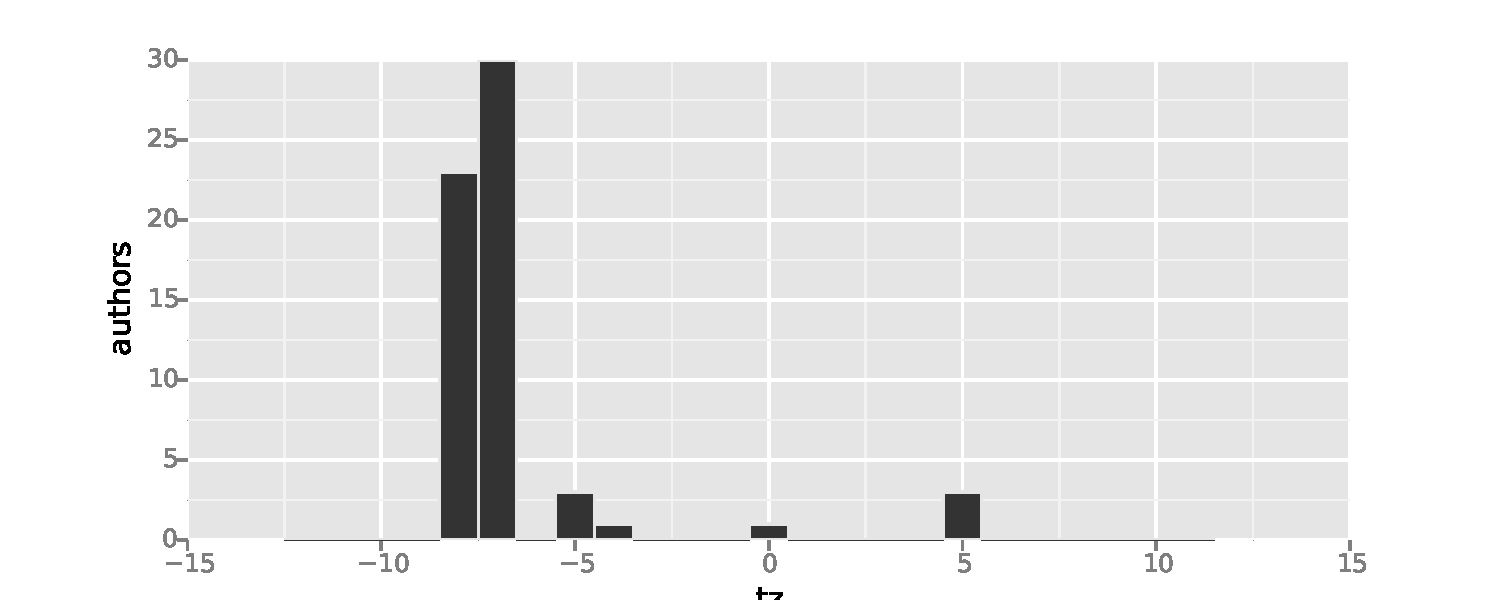
\includegraphics[width=6.9cm]{figs/cloudstack/tz-scm-authors-2010.pdf}
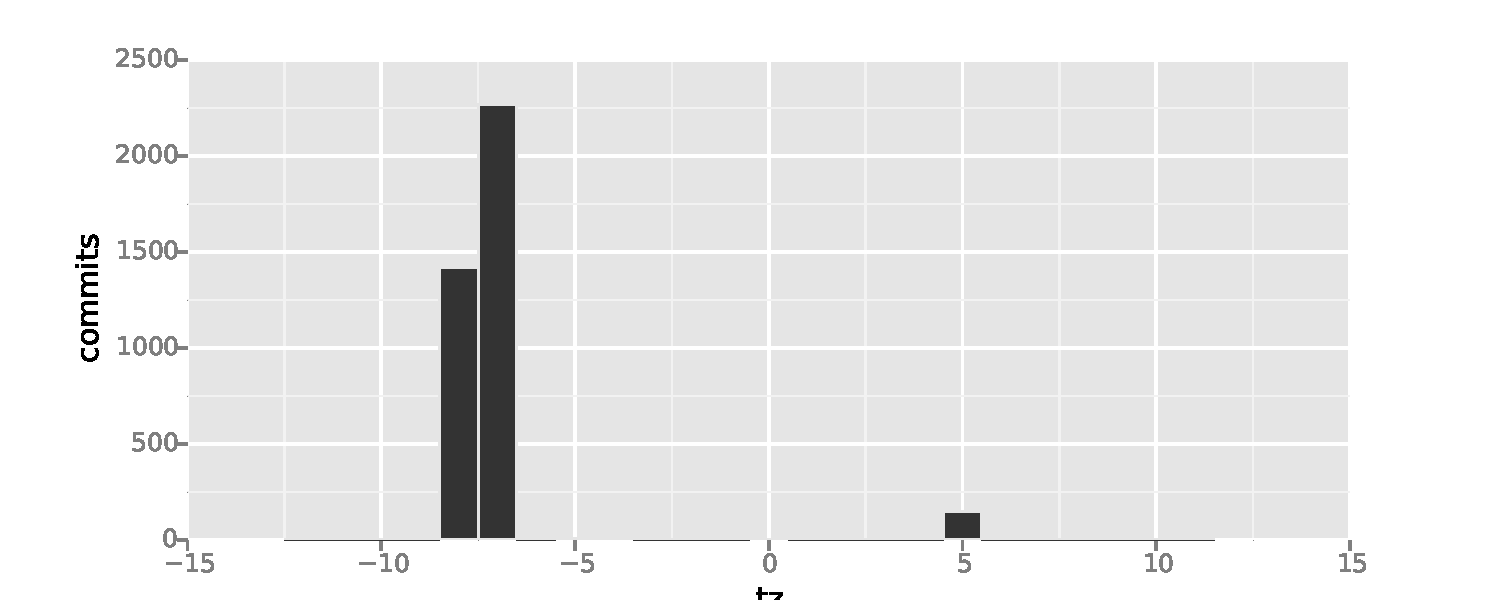
\includegraphics[width=6.9cm]{figs/cloudstack/tz-scm-commits-2010.pdf}
\caption{2010 time-zone analysis for authors (top) and commits (bottom) for
the CloudStack project SCM repository.}
\label{fig:2010-scm}
\end{figure}

Figure~\ref{fig:2014-scm} shows the same analysis for CloudStack's SCM
repository, but this time for the year 2014. As we can see
from the figure at the top, the number of authors has increased significantly
in these four years. In addition, the project is more geographically distributed.
So, on one hand, we can observe authors from all U.S. time zones, although
being the West Coast still predominant. The three European timezones (UTC to UTC+2)
have all over 20 developers, and India (UTC+5) achieves the maximum number
of authors with 55. Developers from other Asian or from Australia are marginally
present too (see UTC+7 to UTC+10).

If we have a look at the bottom figure of Figure~\ref{fig:2014-scm}, we observe
the number of commits by timezone. Here we see that the CloudStack development
is performed in three regions, the U.S. (with a peak in the West), Europe (with
a peak in Eastern Europe, UTC+2) and India (UTC+5).


\begin{figure}[!h]
\centering
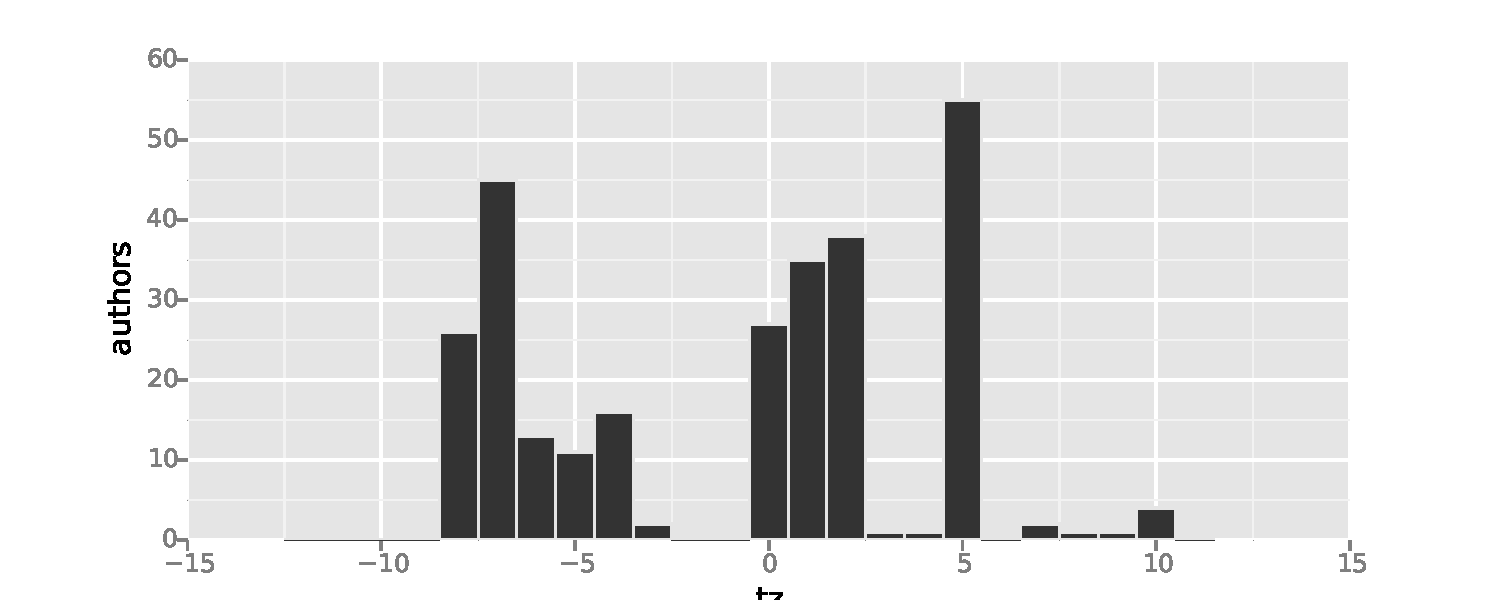
\includegraphics[width=6.9cm]{figs/cloudstack/tz-scm-authors-2014.pdf}
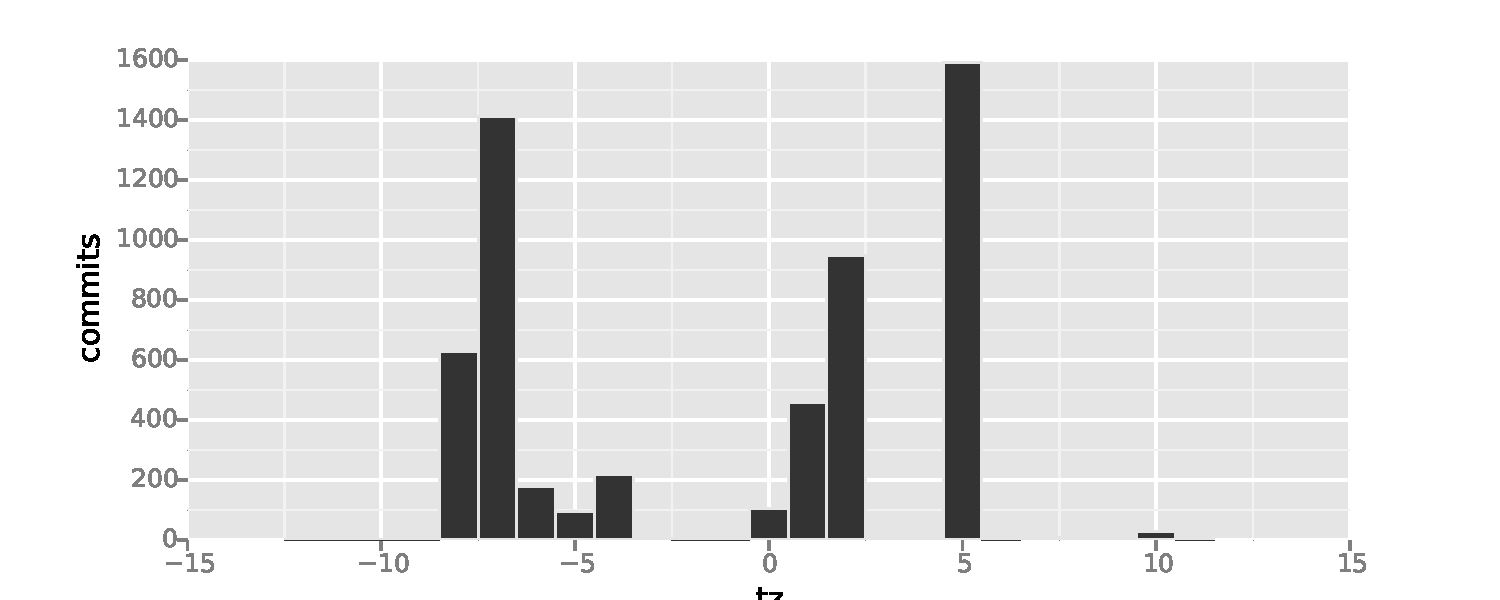
\includegraphics[width=6.9cm]{figs/cloudstack/tz-scm-commits-2014.pdf}
\caption{2014 time-zone analysis for authors (top) and commits (bottom) for
the CloudStack project SCM repository.}
\label{fig:2014-scm}
\end{figure}


\subsection{Analysis of MLs}

Figure~\ref{fig:2012-mls} offers the results for the analysis of the
CloudStack MLs for the year 2012. The vertical axis in the figure
at the top provides the number of different authors, while for the figure
at the bottom it corresponds to number of messages. MLs in 2012 already showed a global distribution
of participants of the CloudStack project, hinting that authorship and activity
in MLs possibly precedes development activity. However, there are
two interesting points that require a specific analysis for themselves: The first
one is the UTC time zone, which includes all authors and activity from countries
such as UK, Ireland or Portugal, but as well all those who use the default
timezone in their mail clients. Therefore, the data for UTC has to be taken 
with care. On the other hand, we have UTC+8, which corresponds to China,
Southeast Asia and Australia's Western Standard Time, among other territories.
That timezone is used by a large number of authors, but few messages have been
sent.

\begin{figure}[!h]
\centering
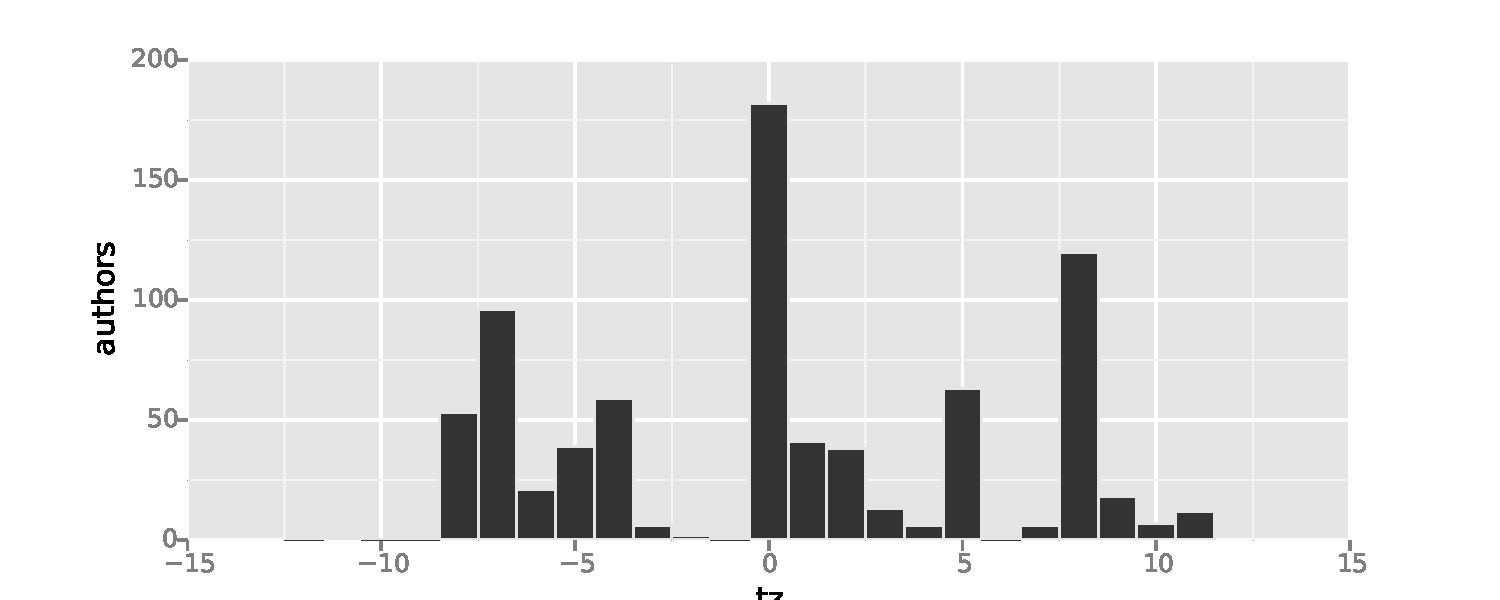
\includegraphics[width=6.9cm]{figs/cloudstack/tz-mls-authors-2012.pdf}
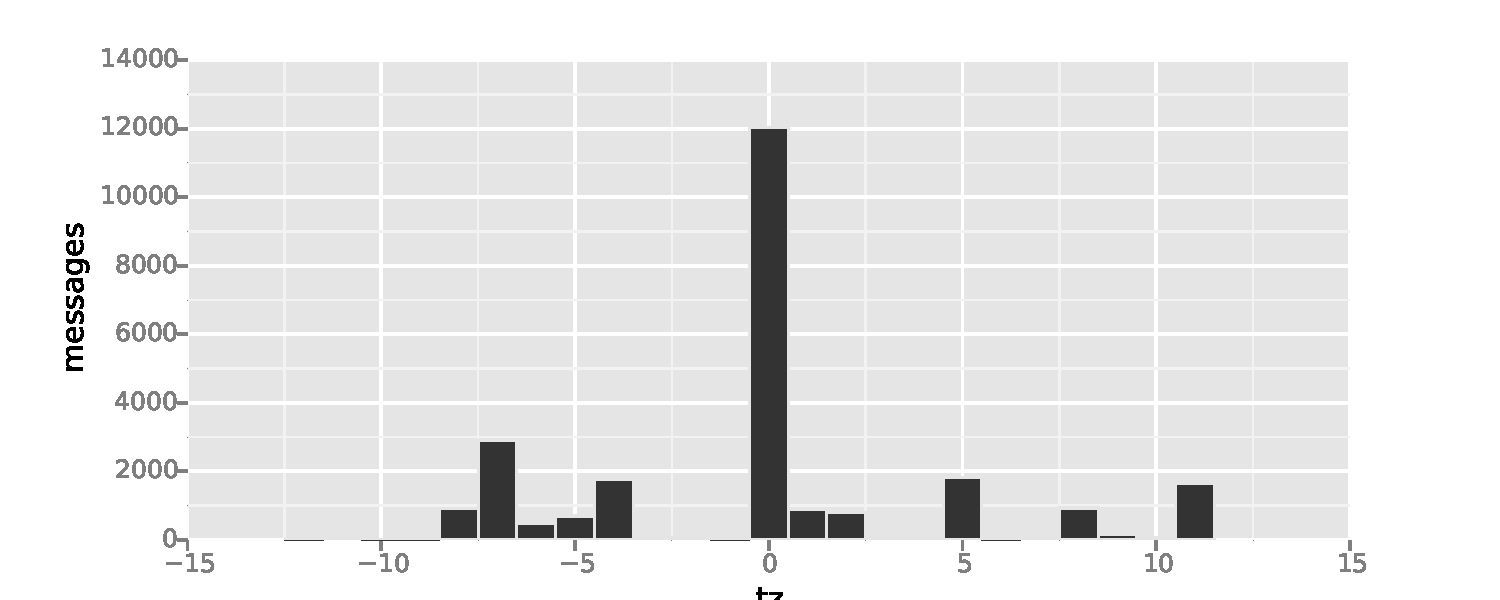
\includegraphics[width=6.9cm]{figs/cloudstack/tz-mls-messages-2012.pdf}
\caption{2012-mls}
\label{fig:2012-mls}
\end{figure}

Figure~\ref{fig:2014-mls} gives the same analysis for MLs,
but this time for number of authors and messages per timezone in the year
2014. Again, UTC is the most significant timezone, which heavily biases results,
which limits the possibility of performing a proper analysis.

\begin{figure}[!h]
\centering
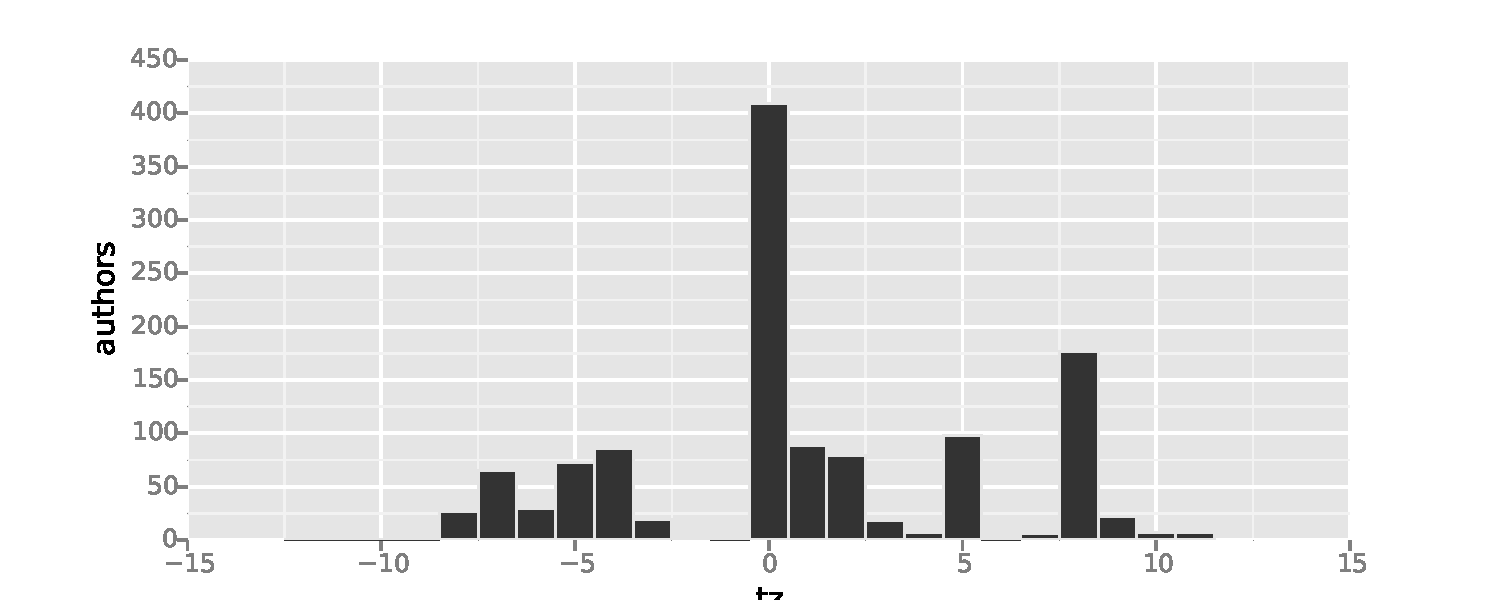
\includegraphics[width=6.9cm]{figs/cloudstack/tz-mls-authors-2014.pdf}
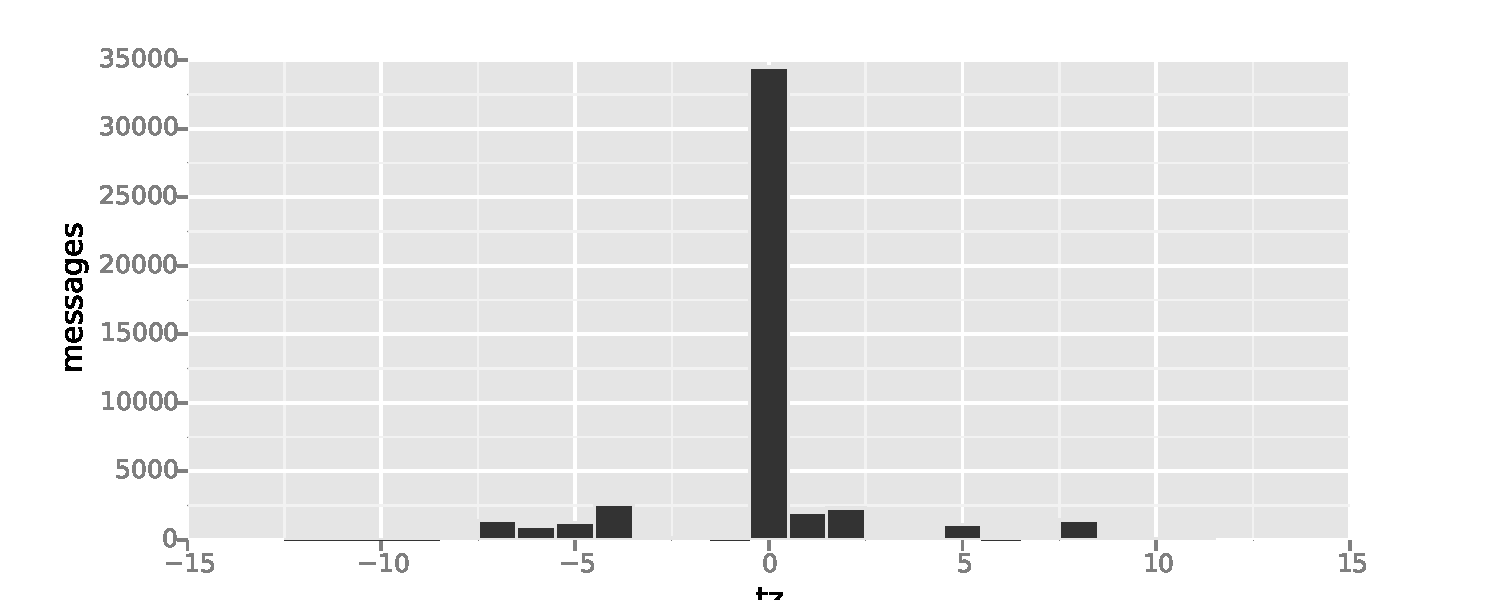
\includegraphics[width=6.9cm]{figs/cloudstack/tz-mls-messages-2014.pdf}
\caption{2014-mls}
\label{fig:2014-mls}
\end{figure}


%-----------------------------------------------------------------------
\section{Discussion}
\label{sec:discussion}

The application of our methodology on the case study has shown that it
is a good to determine if a project is developed and supported globally. 
So, for instance, we could identify that the CloudStack project was
originally developed in a limited geographic zone and has expanded to 
be globally distributed in the last four years. This finding, by itself
is very promising.

On the other hand, the methodology can be fully automated with free software
tools and uses as the
basis for its analysis data that is in general available or can easily be
obtained.

However, there are a number of limitations in the approach that we have
presented:

\begin{enumerate}

  \item There are some territories that have a different time zone during
Winter and Summer. This can be seen visually in our charts with a \emph{shift}
of the bars.

  \item The nature of timezones, comprising several territories makes it
impossible to know, given a time zone, to what specific country (or territory)
the author belongs. So for instance, the Central European time zone includes
from Spain to Poland in Europe, but many African countries as well. Our
original approach for this study was to use a world map instead of stack bars.
However we found that by doing so the results were more easily to be interpreted
in a wrong way.

  \item The UTC+0 configuration problem in email clients includes a severe 
\emph{bias} for this time zone, as it has been shown from the analysis of the
MLs in CloudStack.

  \item We have observed that sometimes obtaining the data for the mailing
list analysis is not straightforward as the archives only store the server
date. Thus, to perform the analysis correctly, the original time and time zone
information has to be preserved.

\end{enumerate}

%-----------------------------------------------------------------------
\section{Conclusions and future work}
\label{sec:conclusions}

In this paper we have presented a methodology that can be used to measure
the globalization of a FLOSS project. Our method is based on data that
is in general publicly available, and that can be analyzed using free software
tools. With the help of a case study, we have seen how we can infer 
information about the geographic dispersion of contributors to the project,
and by doing the analysis on an annual basis, how it changes over time.

As future work we plan to apply this methodology to other projects to find
out if different patterns can be found.

%-----------------------------------------------------------------------
\section*{Acknowledgments}

The work of Jesus Gonzalez-Barahona and Gregorio Robles has been funded in part by the Spanish Gov. under SobreVision (TIN2014-59400-R) and by the Comunidad de Madrid under eMadrid (S2013/ICE-2715). Daniel Izquierdo-Cortazar is supported by the Spanish Gov. with a Torres Quevedo (PTQ-12-05577) grant.



%
% The following two commands are all you need in the
% initial runs of your .tex file to
% produce the bibliography for the citations in your paper.
\bibliographystyle{plain}
\bibliography{biblio}  % sigproc.bib is the name of the Bibliography in this case
% You must have a proper ".bib" file
%  and remember to run:
% latex bibtex latex latex
% to resolve all references
%
% ACM needs 'a single self-contained file'!
%
%APPENDICES are optional
%\balancecolumns

\end{document}
